\documentclass{article}
\usepackage[utf8]{inputenc}
\usepackage{graphicx}
\usepackage{url}
\usepackage[export]{adjustbox}
\usepackage{float}
\usepackage{hyperref}
\graphicspath{ {./images/} }

\title{\large \textbf{ Traffic monitoring\\ Computer networks project \\University "Alexandru Ioan Cuza"  }}
\author{\large \textbf{ Ion Zmeu E4}}
\date{December 8, 2022}

\begin{document}

\maketitle

\section{\textbf{Introduction}}
\hspace{1.5cm}In a world where technology is advancing, it becomes inseparable from normal life, getting into every possible activity that we have cars are not an exception.

\hspace{1cm}Knowing the importance of safe driving, we need programs that are easy to use and provide simplistic but useful features that won't disturb the driver's attention or even help him because safety is the number one priority when you are behind the wheel.

\hspace{1cm}This application has the role of helping each individual driver by delivering personalized useful information such as : the current speed limit or if they got over the speed limit, any incidents that happened and were reported by other drivers, or they can report it by themselves they can also get if wanted sport news, weather or gas prices updates.
\section{\textbf{Used technologies}}
Int sockfd = socket(domain, type, protocol)
\subsection{sockfd}
Socket descriptor, an integer (like a file-handle)\\
\subsection{domain}
Integer, specifies communication domain. We use AF\_ LOCAL as defined in the POSIX standard for communication between processes on the same host. For communicating between processes on different hosts connected by IPV4, we use AF\_INET and AF\_I NET 6 for processes connected by IPV6.But in our case we use only IPV4.\\
\subsection{type} 
communication type\\
\hspace{1.5cm}SOCK\_STREAM: TCP(reliable, connection oriented)\\
\hspace{1.5cm}SOCK\_DGRAM: UDP(unreliable, connectionless)\\
We need a relieable conecction with precise and reliable data so in our case we use TCP(Transmission Control Protocol) even if it is a little bit slower because  a small error could lead to an accident in trafic.
\subsection{protocol}
Protocol value for Internet Protocol(IP), which is 0. This is the same number which appears on protocol field in the IP header of a packet. 
\subsection{Connection}
TCP provides reliable communication by using the 3-way handshake.
\begin{itemize}
  \item Step 1 (SYN): In the first step, the client wants to establish a connection with a server, so it sends a segment with SYN(Synchronize Sequence Number) which informs the server that the client is likely to start communication and with
  \item Step 2 (SYN + ACK): Server responds to the client request with SYN-ACK signal bits set. Acknowledgement(ACK) signifies the response of the segment it received and SYN signifies with what sequence number it is likely to start the segments with
  \item Step 3 (ACK): In the final part client acknowledges the response of the server and they both establish a reliable connection with which they will start the actual data transfer
\end{itemize}
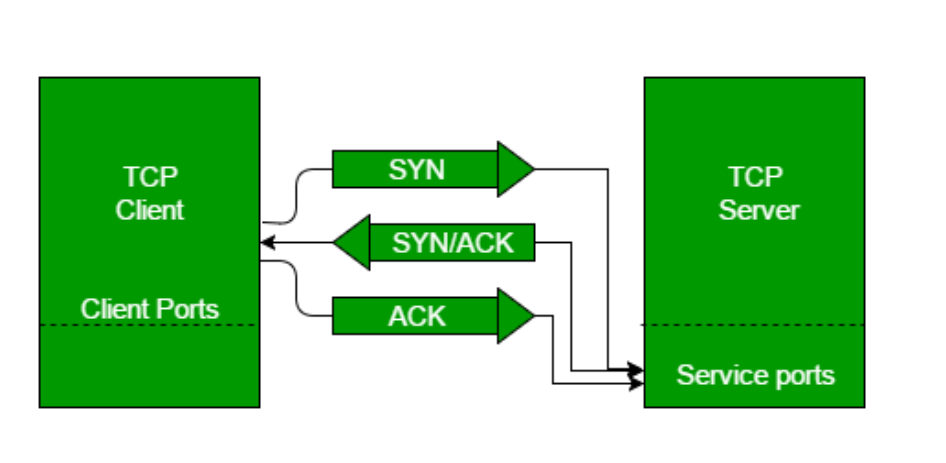
\includegraphics[width=125mm,height=60mm]{3way}\\
\clearpage
\section{\textbf{Application architecture}}
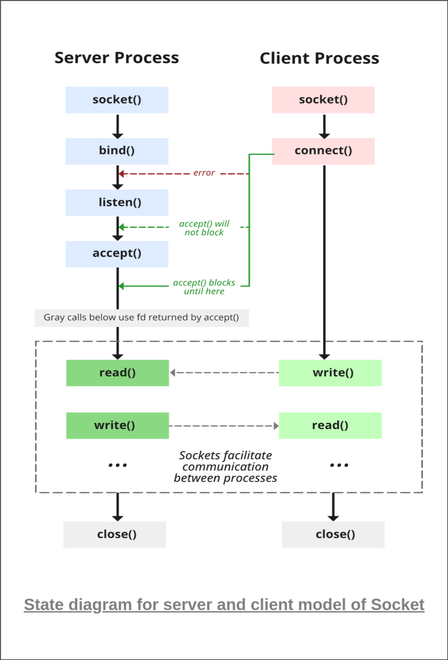
\includegraphics[width=125mm,height=180mm]{tcp}\\
\break
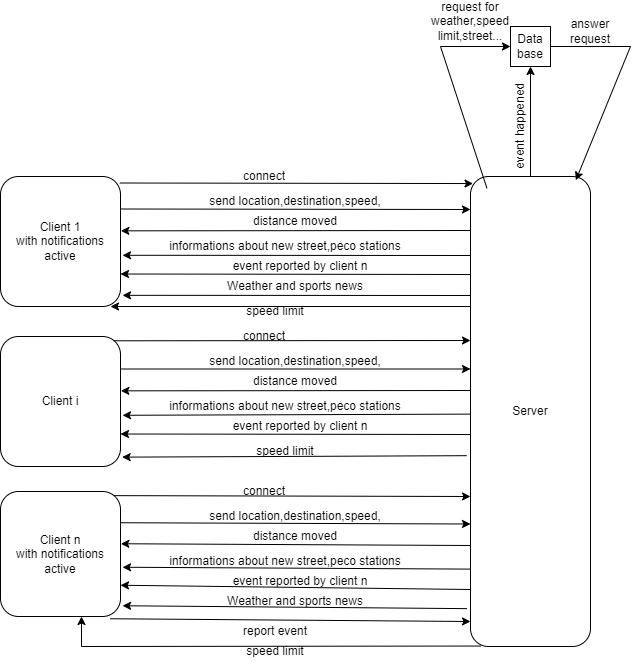
\includegraphics[width=125mm]{sch}\\

\section{\textbf{Implementation details}}
The server will create threads to communicate in a concurent way with all the clients.The server waits for clients to request a connection and once found it creates a thread to communicate with them .\\
Communication with the clients start with recieving informations like : the starting location,the destination,recieve or not notifications about gas prices , sport news and weather updates,and also a information that can be used to log the user in the system.\\
Notifications about gas prices , sport news and weather updates will be sent from server to the client at the start of its ride and also when he enters a new street if the client will request them at the start of his ride.\\
In this structure we will have information that the client will send to our server.\\
\begin{verbatim}
typedef struct thData{
	int idThread; //id-ul thread-ului tinut in evidenta de acest program
	int cl; //descriptorul intors de accept
	int speed;//viteza de circulatie
	char loginfo[100];//informatie pentru logare
	char currnet[100]; // strada pe care circula 
	char start[100]; // punctul de plecare
	char end[100]; //destinatia
	bool notify;// notificari
\end{verbatim} 

After recieving this information the server will do a couple of checks to make sure everyrhing is correct for example the start and end streets should be different,and it also sends information about the gas prices ,sport news and weather updates if the client turned notifications on.Also when the client enters a new street it will send the street name to the server and the speed it drives and the server will respond with information about gas prices and a warning of speeding if it is the case or just tell the client the current speed limit ,the client will also send the server its speed from time to time. \\
\subsection{Report an event}
When a driver send an report it goes from the client to the server which sends coresponding information to all the clients and limiting the speed limit on the specific street by 20km/h.
\subsection{Notifications}
If the notifications are requested by the client then the news and weather updates are sent to them and may be updated when the client enters another street,gas price will be updated based on the street which the client entered in case the street has a Peco station and will respond when there aren't any correspondingly.
\subsection{New street}
When the client enetrs a new street it will send the name of the street to the server which will return informations about the peco gas stations and notifications if needed.
\subsection{Speed}
Server recieves the speed periodically from the clients to which he responds with warnings in case the client is too slow or too fast on the current street.
\subsection{End connection}
When the client arrives at its destination or the connection is ended prematurely the server will be notified and it will close the connection with the client.The thread will close and the space occupied by it will be freed.
\subsection{Client}
Client is fast and easy to use to help the driver communicate with the server and it will check the information given by the driver to make sure that the server gets only correct and usefull information. 
\section{\textbf{Conclusions}}
The application uses TCP to make sure there are no errors when the information exchange between the client and server takes place .It is made to be easy to use for the driver and provide with personalized and usefull information while also offering some functions that will help increase the safety of the driver by providing the speed limit and exceptional events that happened on its route.The server will also save all the information such as the streets , speed limits,events,weather ,sport news and peco station gas prices in a database. 


\section{\textbf{Bibliography}}
\url{https://www.geeksforgeeks.org/udp-server-client-implementation-c/} \newline
\url{https://www.geeksforgeeks.org/socket-programming-cc/} \newline
\url{https://www.geeksforgeeks.org/tcp-3-way-handshake-process/} \newline
\url{https://profs.info.uaic.ro/~computernetworks/cursullaboratorul.php} \newline
\url{https://maps.google.com/} \newline
\url{https://www.tutorialspoint.com/sqlite/sqlite\_c\_cpp.htm} \newline
\url{https://profs.info.uaic.ro/~computernetworks/ProiecteNet2022.php} \newline



\end{document}
